 \chapter[Niche Use and Conservation in \textit{Aedes} Arbovirus Vectors]{Niche Use and Niche Conservation Under Climate, Habitat and Resource Constraints for Two Global Arbovirus Vectors}

Christopher B. Anderson\textsuperscript{1,2},
Erin A. Mordecai\textsuperscript{1},
Meghan E. Howard\textsuperscript{1},
Luis E. Fernandez\textsuperscript{3,4},
Ricardo Gamboa\textsuperscript{5},
Marcelo Guevara\textsuperscript{6},
Morgan P. Kain\textsuperscript{1,6},
Andres G. Lescano\textsuperscript{7},
Lisa Mandle\textsuperscript{6},
Stephanie Montero\textsuperscript{7},
Mileyka Santos\textsuperscript{8},
Jeffrey R. Smith\textsuperscript{1,2},
Adrian Vogl\textsuperscript{6},
and Gretchen C. Daily\textsuperscript{1,2,6,7} \\[6pt]

\noindent\textsuperscript{1}\small{Department of Biology, Stanford University, Stanford, USA}

\noindent\textsuperscript{2}\small{Center for Conservation Biology, Stanford University, Stanford, USA}

\noindent\textsuperscript{3}\small{Centro de Innovación Científica Amazónica (CINCIA), Puerto Maldonado, Perú}

\noindent\textsuperscript{4}\small{Center for Energy, Environment, and Sustainability, Wake Forest University, Winston-Salem USA}

\noindent\textsuperscript{5}\small{School of Public Health and Administration, Universidad Peruana Cayetano Heredia, Lima, Perú}

\noindent\textsuperscript{6}\small{Natural Capital Project, Stanford University, Stanford, USA}

\noindent\textsuperscript{7}\small{Woods Institute for the Environment, Stanford University, Stanford, USA}

\noindent\textsuperscript{8}\small{Department of Medical Entomology, Gorgas Memorial Institute of Health Studies, Panama City, Panamá}

\section{Abstract}

Mosquitoes are expected to shift their geographic distributions with rising temperatures, urbanization, agricultural expansion and human population growth. As ectotherms, temperature responses are mechanistically understood for many mosquito arbovirus vectors, but the mechanisms driving other environmental responses are not. How do these covarying environmental changes interact to shift future distributions of vectors? Here, we quantified how three distinct dimensions of the vector niche—climate, habitat, and resource constraints—interact to determine the distributions of two mosquito species, \textit{Aedes aegypti} and \textit{Ae. albopictus}, which transmit dengue, chikungunya, Zika, and other viruses across Latin America and the Caribbean. When considered independently from other drivers, resource constraints (i.e., access to blood meals) best predicted the realized niche for \textit{Ae. aegypti}, while temperature constraints best predicted niche patterns for \textit{Ae. albopictus}. Both vectors occurred disproportionately in areas with high mean and low variance in temperature throughout the year, revealing strong niche preferences for high temperatures and thermal stability. \textit{Ae. aegypti} was more frequently observed at warmer temperatures (mean = 31.0$\degree\, C$) than \textit{Ae. albopictus} (mean = 29.1$\degree\, C$), consistent with mechanistic predictions of vector-specific thermal optima. \textit{Ae. aegypti} occurred in areas of higher population density (mean = 632.2 $people\, km^{-2}$) than \textit{Ae. albopictus} (mean = 363.6 $people\, km^{-2}$), which tended to occur in areas of higher livestock density (mean = 4.4 $animals\, km^{-2}$). Resource use patterns were consistent across Mesoamerica, South America, and the Caribbean for both vectors, while climate and habitat patterns were region-specific, suggesting \textit{Aedes} distribution patterns may be constrained by access to blood meal.

\section{Introduction}

The global burden of dengue is increasing worldwide, with the number of symptomatic infections doubling every decade since 1990 \cite{Stanaway2016-mo}. The geography of transmission is expected to shift under climate change \cite{Bhatt2013-qa, Campbell2015-ky}, increasing in temperate areas and decreasing in areas that will become too hot to support sustained viral transmission \cite{Mordecai2019-ya, Ryan2019-pz}. These shifts may be especially pronounced in Latin America and the Caribbean \cite{Shepard2011-nz, Tapia-Conyer2012-yw}, which have seen rising temperatures, shifting precipitation regimes, and rapid forest loss, each of which promote dengue transmission \cite{Locatelli2011-de, Marengo2011-jk, Collins2013-zo, Nobre2016-jn}. Reduced vector control practices after the 1960s \cite{Gubler2002-af, Gomez-Dantes2009-iu} and human-assisted migration of mosquitoes also drove reintroductions and new invasions across the region \cite{Knudsen1995-pc, Rossi1999-sr, Tatem2006-qu, Ortega-Morales2016-jd}. Recent events indicate short-term increases in transmission as well: Perú announced a dengue emergency for three Amazonian departments in February 2020 \cite{Ministerio_de_Salud_Peru2020-pb, US_Embassy_Lima2020-gd} and Brazil reported nearly 1.5 million dengue cases in the 2019 dry season alone—more than all cases reported in 2017 and 2018 combined \cite{Brazil2019-xb, Pan_American_Health_Organization_World_Health_Organization2020-ov}.

The globally invasive mosquito species \textit{Aedes aegypti} and \textit{Ae. albopictus} are the primary vectors of dengue, as well as Zika and chikungunya viruses, which caused explosive epidemics in Latin America and the Caribbean in 2016-2017 and 2014-2015, respectively. With no vaccines widely available for these viruses (collectively called arthropod-borne viruses or “arboviruses”), forecasting and intervention are key mitigation strategies \cite{Tapia-Conyer2012-yw, Altizer2013-dn, Castro2019-jb}. As transmission is driven by species interactions between humans and mosquitoes, and moderated by environmental conditions \cite{Hopp2001-zf, Paaijmans2013-dg, Mordecai2019-ya}, transmission forecasts depend to a large degree on how well we can characterize human-vector-environment interactions.

There are two main approaches to modeling how humans and the environment determine mosquito biogeography \cite{Tjaden2018-zi}. Mechanistic models explicitly define the biological and ecological processes driving vector life cycles and infection patterns \cite{Costa2010-cx, Carrington2013-qp, Mordecai2013-sb}. Quantifying the temperature dependence of these processes has been a central focus for ecological epidemiologists, with both lab experiments and mathematical models predicting that mosquito life history and interaction traits vary directly and nonlinearly with temperature \cite{Brown2004-cw, Mordecai2017-tb, Shocket2018-xi}. However, it is unclear whether these thermal responses, alone or in combination with other drivers, predict vector biogeography with the same precision \cite{Tjaden2018-zi}. Alternatively, species distribution models (SDMs) characterize biogeographic patterns of where species are present, using occurrence records and environmental data to quantify a species’ realized niche (the conditions of occupied habitat) and to predict its fundamental niche (potentially suitable habitat), though these methods eschew mechanism for predictive power \cite{Grinnell1917-aa, Soberon2005-cn, Wiens2009-sb}. Global SDMs for \textit{Ae. aegypti} and \textit{Ae. albopictus}, and for the arboviruses they transmit, report that temperature and precipitation are the predominant drivers of vector biogeography and are the best predictors of epidemic potential \cite{Brady2014-ti, Liu-Helmersson2014-cd, Kraemer2015-ct}, corroborating mechanistic models. Recent studies have merged these approaches by applying lab-derived thermal responses to climate-driven niche maps to forecast spatial transmission patterns \cite{Tjaden2017-af, Mweya2016-cv}. 

Despite this consistency between mechanistic and statistical methods, it’s not yet clear that climate alone sufficiently characterizes the mosquito vector niche. Spatially-explicit cross-validation studies suggest it may not \cite{Liu2020-wk}. Multiple climate-driven SDMs for \textit{Ae. aegypti} and \textit{Ae. albopictus}, trained on data from Asia, Europe and North America, have failed to generalize to Latin America where both vectors are invasive, suggesting that vector-climate relationships are not consistent across continents \cite{Medley2010-fa, Carlson2016-rc, Pech-May2016-vs}. These results have been interpreted as evidence of niche evolution; that each vector is adapting to new climates as it invades. But niche evolution is a complex process, and climate constraints only characterize one dimension of the vector niche \cite{Wiens2010-ce, Hortal2015-gc, Diniz-Filho2019-cd}. Moreover, no direct evidence exists to support the idea that vector thermal constraints are evolving. Is it instead possible that other conserved ecological mechanisms, like habitat or resource constraints, better explain spatial invasion patterns?

\textit{Aedes} habitat constraints are typically characterized by land cover, with \textit{Ae. aegypti} often found in vegetated urban areas \cite{Troyo2009-yv, Jansen2010-uj} and \textit{Ae. albopictus} found in rural and agricultural areas \cite{Knudsen1995-pc, Tsuda2006-gl}, though the urban/rural dichotomy does not always hold \cite{Li2014-fq}. In global models, the importance of climate overshadows land cover when solely characterized by simple remote sensing metrics \cite{Kraemer2015-ct, Carlson2016-rc}. Yet land cover better describes vector distributions when represented by descriptive metrics like vegetation phenology, tree cover, or building density, which mechanistically map to access to sugar feeding resources, natural breeding sites, or urban breeding sites, respectively \cite{Martinez-Ibarra1997-ra, Peterson2005-ml, Vanwambeke2007-pw, Troyo2009-yv, Landau2012-dn, Li2014-fq}. These hematophagous vectors are also reproductively constrained by access to blood meals \cite{Padmanabha2012-xa}. Humans are the primary blood meal source for both vectors, but \textit{Ae. albopictus} is less specific and will often feed on domesticated mammals and on wildlife \cite{Gratz2004-xn, Delatte2008-hc}. Despite the outsized importance of resource constraints in other ecological contexts, they are rarely quantified when mapping \textit{Aedes} niche use. We hypothesize that spatial invasion patterns that are unexplained by climatic constraints may instead be explained by habitat or resource constraints.

In this paper we quantified niche preferences and evaluated evidence for niche conservation in \textit{Ae. aegypti} and \textit{Ae. albopictus} in Latin America and the Caribbean, where both vectors are invasive. We asked:

\begin{enumerate}
    \item To what degree do climate, habitat, and resource constraints predict spatial patterns of niche use for \textit{Ae. aegypti} and \textit{Ae. albopictus} at continental scales? 
    \item How do statistically-derived niche preferences compare to direct lab and field observations?
    \item Are climate, habitat, and resource preferences conserved across Latin America and the Caribbean for each vector?
\end{enumerate}

\noindent We trained presence-only SDMs using 11 mechanistically-based covariates to quantify the importance of three niche dimensions (climate, habitat, and resource constraints) in characterizing each vector’s realized niche. We compared our results to lab-derived thermal responses and two field surveys of vector abundance to reconcile biogeographic and experimentally-derived patterns. To evaluate evidence of niche conservation, we tested whether models trained in one region predicted spatial distributions in other regions. We took a novel approach to adjusting for sampling bias—assuming sampling effort was biased towards urban areas—using a global nightlights dataset and non-\textit{Aedes} occurrence records from the Culicidae family per the target group background selection method \cite{Phillips2009-nf, Merow2013-mw}. This is distinct from studies that solely restrict background sample selection to vector-specific envelopes of temperature suitability \cite{Brady2014-ti, Kraemer2015-ct}. We exclusively used satellite-derived covariates, which provide spatially continuous and regularly-spaced measurements instead of interpolated weather station data, which are sparse across Latin America and the Caribbean \cite{Fick2017-am}.

\begin{figure}[!ht]
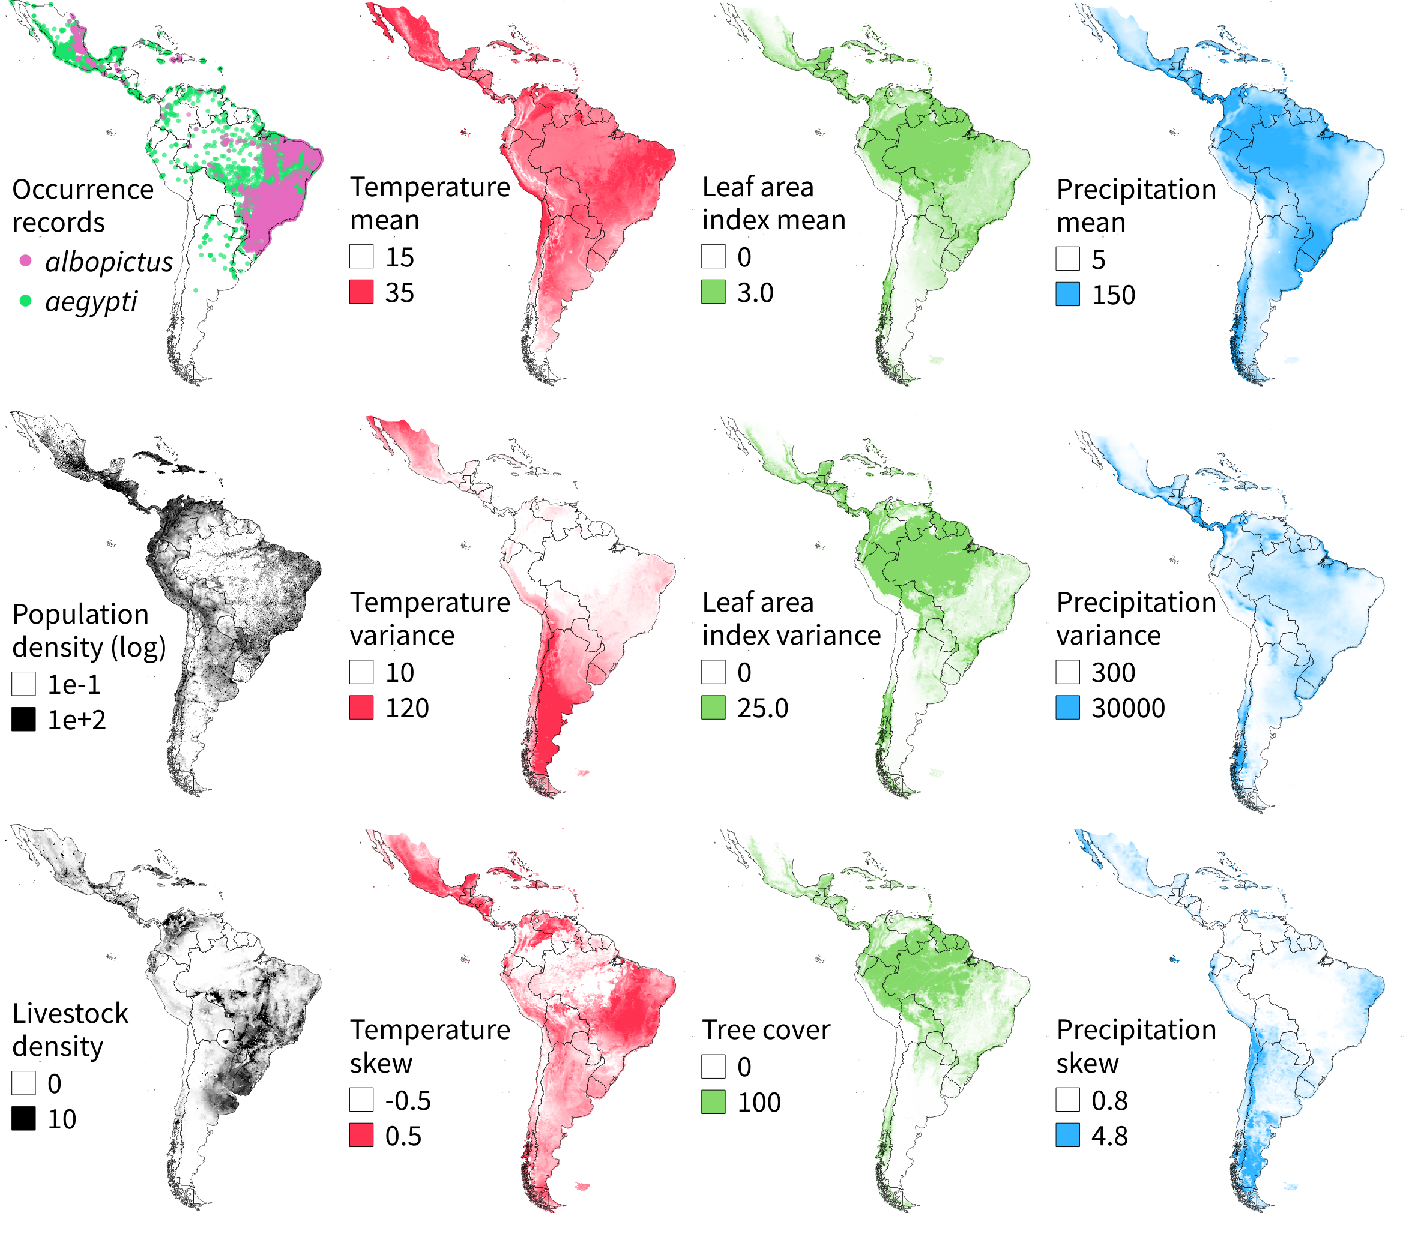
\includegraphics[width=\textwidth]{figures/ch3-map-covariates.pdf}
\centering
\caption[Species occurrence records and environmental covariates show continental-scale niche use patterns that determine \textit{Aedes} distributions.]{Species occurrence records and environmental covariates show continental-scale niche use patterns that determine \textit{Aedes} distributions. The human population density map (black, top) was $log_10$ transformed from units of $people\, ha^{-1}$. The livestock density map (black, bottom) is in units of $animals\, km^{-2}$. Temperature patterns (red) are reported in $\degree C$. Leaf area index patterns (green, top) are reported in units of $m^2\, m^{-2}$, while tree cover (green, bottom) is reported in $\%$. Precipitation patterns (blue) are reported in units of $mm\, mo^{-1}$.}
\label{fig:map-covariates}
\end{figure}

\section{Methods}

Species distribution modeling is based on the Grinellean niche concept: the environmental conditions that allow individuals of a species to survive and reproduce will constrain the distributions of those species \cite{Grinnell1917-aa, Wiens2009-sb}. The inputs to these models are spatially explicit species occurrence records and gridded environmental covariates, which we gathered and derived from publicly-accessible datasets (Fig. \ref{fig:map-covariates}). We also included a bias assessment in our models, described in-depth below, as \textit{Aedes} records are often collected in populated areas in efforts to map human disease risk. We sampled background covariates in proportion to the sampling effort of the occurrence data (i.e., we assessed suitability relative to the environmental conditions where sampling was most likely to occur). All spatial data were projected to a Molleweide global equal area, $1\, km^2$ grid prior to analysis (EPSG:54009), all map figures made in web mercator (EPSG:3857), all scripts can be found on GitHub (https://github.com/earth-chris/aedes-americas), all species distribution models were trained using the Maxent software \cite{Steven_J_Phillips_Miroslav_Dudik_Robert_E_Schapire_undated-nv}, and all spatial analysis was performed in Python or on Google Earth Engine \cite{Gorelick2017-nx}.

\subsection{Occurrence Records and Environmental Covariate Data}

We analyzed 6,317 \textit{Aedes aegypti} occurrence records and 3,629 \textit{Ae. albopictus} records from two global datasets: the Global Biodiversity Information Facility (GBIF; https://gbif.org) and from a global synthesis by \cite{Kraemer2015-sm}. All data were filtered to contain only records in Latin America and the Caribbean from 2000 to 2017. Raw \textit{Ae. aegypti} data from GBIF contained 5,648 records \cite{Gbif2018-ae}, and the raw \textit{Ae. albopictus} data contained 3,452 records \cite{Gbif2018-aa}. All GBIF data were cleaned to include only published records, to exclude points with $>$ 10 km reported spatial uncertainty, and to include only points recorded by human observation. The raw \textit{Ae. aegypti} data from Kraemer et al. contained 1,067 records, and the raw \textit{Ae. albopictus} data contained 159 records, which were quality checked prior to publication \cite{Kraemer2015-sm}. The GBIF and Kraemer et al. data were cleaned to remove duplicate records, and reprojected to the global equal area grid. To reduce spatial autocorrelation effects, we created a 5x5 km grid and only included one randomly selected record from grid cells with more than one record \cite{Segurado2006-gy, Hawkins2012-gu}.

To assess the relative importance of climate, habitat and resource constraints on niche use, we developed satellite-derived metrics that capture the spatial and temporal variation in temperature, precipitation, land cover and population densities. The spatial and temporal scales over which these patterns vary are quite distinct. While land cover can vary greatly over small spatial scales, it typically varies only minimally within a year in undisturbed landscapes. If land cover does change within a year, it’s often the result of a transformative process (e.g., the conversion of forest to pasture). In contrast, temperature and precipitation can vary greatly on daily and monthly time scales, but at any time the spatial turnover in these patterns can be small relative to turnover in land cover. The derived covariates attempted to capture and fairly represent these spatial and temporal dynamics across scales for these niche constraints.

For temperature and precipitation, we derived mean, variance, and skewness statistics on a per-grid cell basis using all daily MODIS land surface temperature (LST; $\degree\, C$) and hourly TRMM precipitation measurements (PCP; $mm\, mo^{-1}$) from 2002-2017 \cite{Justice1998-pu, Huffman2007-iu, Hou2013-cn}. We calculated mean temperature and precipitation metrics to identify preferences for average conditions over a year, variance metrics to identify preference for static or dynamic climatic conditions, and skewness to calculate preference for anomalously hot/cold or wet/dry conditions \cite{Huffman2007-iu, Hou2013-cn}. We included three land cover metrics to characterize habitat constraints: tree cover (TC; $\%$) and the mean and variance of leaf area index (LAI; $m^{2}\, m^{-2}$) from 2002-2017 \cite{Justice1998-pu, Hansen2013-oz}. The LAI covariates were selected to describe vegetation growth and phenology, as well as access to sugar feeding resources \cite{Martinez-Ibarra1997-ra, Chen2015-dw}. Tree cover was included to distinguish forests from agriculture and because each vector uses trees in urban and agricultural landscapes as habitat \cite{Troyo2009-yv, Landau2012-dn}. To characterize resource constraints (i.e., available blood meal), we analyzed two population density covariates, human population density (POP; $people\, km^{-2}$) and livestock density (LIV; $animals\, km^{-2}$) from WorldPop and the Gridded Livestock of the World database \cite{Tatem2017-ma, Gilbert2018-bm}. Human population density was log\textsubscript{10} transformed to increase normality prior to analysis.

\subsection{Species Distribution Modeling}

To address our first research question, we evaluated niche preferences using the Maxent species distribution modeling software \cite{Phillips2006-ua, Steven_J_Phillips_Miroslav_Dudik_Robert_E_Schapire_undated-nv}, which uses logistic regression to calculate habitat suitability based on the conditional density of features at occurrence points and the unconditional density of features across the study area \cite{Elith2011-kb}. Prior to analysis, we used the target group selection method \cite{Phillips2009-nf, Merow2013-mw} to generate a sampling bias adjustment using non-\textit{Aedes} occurrence data from the Culicidae family and urbanization data from nighttime lights \cite{Mills2013-yb}. We used these data to train a Maxent model, then used the cumulative output, which indicates sampling frequency in human populations, as our sampling bias for all other Maxent analyses. We therefore assumed that neither the mosquito vectors nor the vector sampling efforts were uniformly distributed, but biased towards urban centers, so suitability was calculated relative to a statistically-derived null distribution of areas where people live.

Maxent calculates relative species occurrence probabilities by comparing the statistical distributions of environmental covariates at occurrence sites to a similar covariate distribution across potentially accessible habitats (i.e., the background) per Eqn. 4.1:

\begin{equation}
Pr(y=1|z) = 
\frac{f_1(z) \cdot Pr(y=1)}{f(z)}
\end{equation}

Where $y$ represents a species, $y=1$ are locations where that species was observed, $z$ is a vector of environmental covariates, $f(z)$ is a probability distribution of non-linear feature transformations derived from the vector of covariates across the background, $f_1(z)$ is a probability distribution of features derived from the covariates at species occurrence locations, and $Pr(y=1|z)$ is the probability that a species occurs at a point on the landscape as conditioned by the environment. The sampling bias adjustment modified the locations from which the distribution $f(z)$ was drawn.

To identify which environmental covariates independently best predicted \textit{Aedes} niche use, we ran four sets of Maxent models, each using just the covariates from each potential niche axis (i.e., temperature, precipitation, resource availability, and habitat). For population density we set $z = [log10(POP), LIV]$, for temperature we set $z = [LST_{mean}, LST_{var}, LST_{skew}]$, for land cover we set $z = [LAI_{mean}, LAI_{var}, TC]$, and for precipitation we set $z = [PCP_{mean}, PCP_{var}, PCP_{skew}]$. We evaluated model performance using the area under the receiver operator curve (AUC), a metric of separability, which calculates the probability that model predictions distinguish between suitable habitat and a semi-random geographic sample (i.e., the background). We assessed model performance using 4-fold cross validation and reported a modified AUC calculation (described in more detail below).

To assess the relative importance of each environmental covariate, we ran Maxent models using all covariates, setting $z = [log10(POP), LIV, LST_{mean}, LST_{var}, LST_{skew}, LAI_{mean}, LAI_{var}, TC, PCP_{mean}, PCP_{var},\\ PCP_{skew}]$, and reported permutation importance scores. During model fitting, Maxent calculates how model performance changes as feature coefficients change \cite{Phillips2008-ic}. Permutation importance scores are calculated by randomly altering the values of a single covariate and recalculating model performance (here, AUC). These values are rescaled to a percentage based on how model performance changed for each covariate permutation. The mean cross-validation permutation scores are reported in Table B.2.

Maxent models were run with the following parameters. For feature selection we ran models with only ‘hinge’ features enabled, which construct smooth, nonlinear response curves akin to a generalized additive model \cite{Hastie2004-bw, Elith2011-kb}. This was based on the assumption that \textit{Aedes} vectors would respond in a continuous, nonlinear fashion to climate, habitat and resource patterns, akin to other temperature-dependent models that assume unimodal response functions \cite{Mordecai2017-tb}. To reduce model overfitting and to reduce the effects of collinearity in our environmental covariates, we increased the default $\beta$ regularization parameter to 1.5, which penalizes complex models and shrinks model coefficients during training \cite{Merow2013-mw}. We selected this value by minimizing the difference between training and testing AUC scores in cross-validation using models trained with all covariates. For background selection, we preferentially sampled 10,000 random points using the sampling bias map described above. For the output format, we report Maxent’s cumulative suitability metric, which is a relative occurrence rate rescaled between 0 and 100. This output can be interpreted as an omission rate; setting a threshold at a value of 10 to predict presence/absence will omit approximately 10\% of presence records \cite{Phillips2008-ic, Merow2013-mw}.

In our results we report a modified AUC score. AUC can be interpreted as the probability that a randomly chosen presence sample is ranked above a randomly chosen background sample. These probabilities are typically assessed using all test samples for presence and background points. However, when the number of background samples is greater than the number of presence samples, AUC values may appear artificially high by predicting low suitability across a large number of background samples without actually calculating appropriately high suitability scores in the small number of locations where a species is present. This is akin to a zero-inflation effect. We reduced this inflation effect by randomly selecting the same number of background samples as presence test samples (i.e., balancing the test dataset) before calculating AUC scores. This process was bootstrapped 5 times for each model to get an unbiased estimate of the adjusted AUC value, and we reported the bootstrapped mean.

\begin{figure}[!ht]
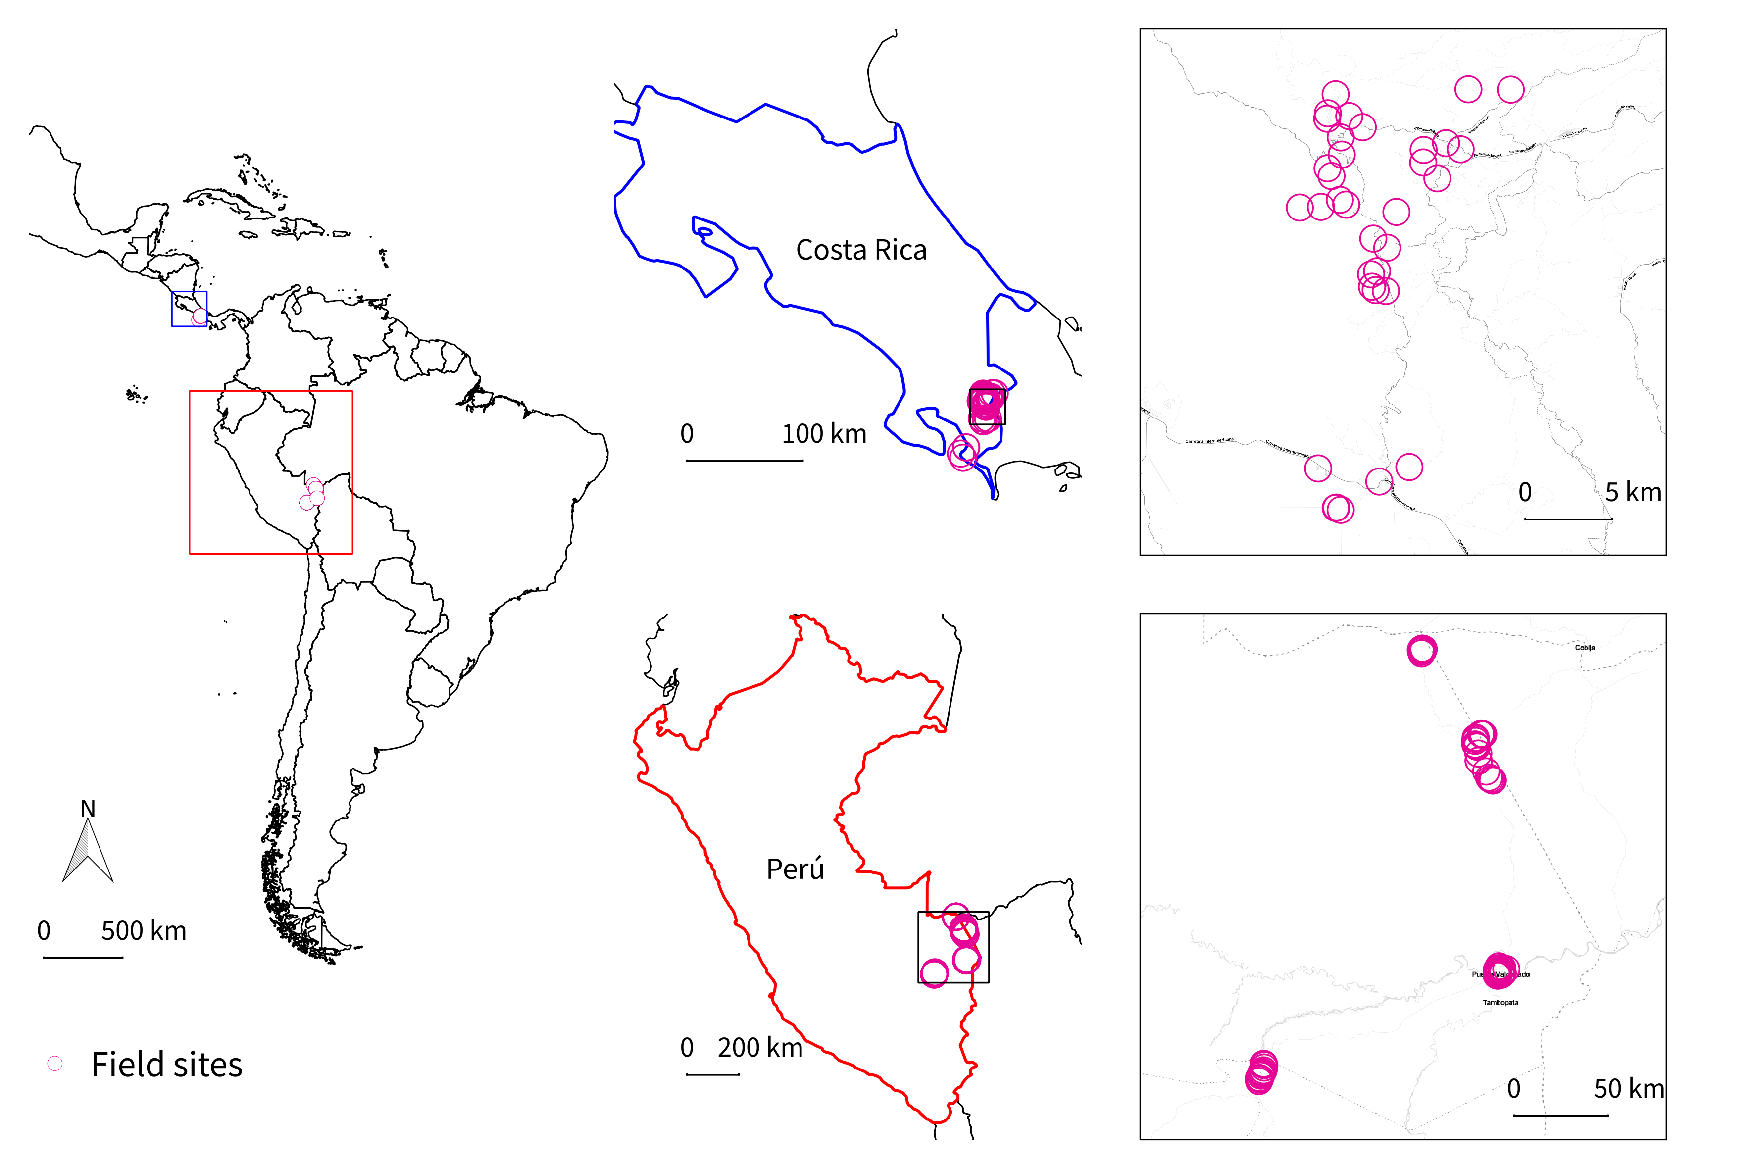
\includegraphics[width=\textwidth]{figures/ch3-map-field.pdf}
\centering
\caption[Field plot locations in Perú and Costa Rica.]{Field plot locations in Perú and Costa Rica. 134 field sites were visited, 38 in Costa Rica (top) and 96 in Perú, where four methods of mosquito trapping were used. These included BG-Sentinel traps, CDC light traps, Gravid \textit{Aedes} traps (GAT), and aspiration. All sites were visited twice, with the exception of four sites in Costa Rica, which were visited once.}
\label{fig:map-field}
\end{figure}

\subsection{Field Data Collection}

To address our second research question comparing model results to field observations, we collected mosquito abundance data using an array of trapping methods across two regions, which included 38 field sites in Costa Rica and 96 field sites in Perú (Fig. \ref{fig:map-field}; Table \ref{tab:plot-locations}). Both regions were sampled during the wet season—July 2017 in Costa Rica and November 2018 in Perú—when \textit{Aedes} vectors and local mosquito surveillance programs were both active. The Costa Rica sites were located in the tropical southeast of the country near the border with Panamá, then considered a southern frontier for \textit{Ae. albopictus}, which hadn’t yet been formally reported in the region despite a recent increase in dengue cases \cite{Gutierrez2015-hx}. The Perú sites were all located in the southeastern department of Madre de Dios. These included a set of sites near the border of Brazil and Bolivia, where there is concern that \textit{Ae. albopictus} could migrate into Perú with traffic along the Interoceanic Highway. \textit{Ae. albopictus} was the predominant vector of interest in the Costa Rica sites, with just three \textit{Ae. aegypti} individuals identified there. \textit{Ae. aegypti} was the only vector of interest identified in the Perú sites.

The site sampling scheme was designed to understand how \textit{Aedes} habitat preferences and abundance patterns change along a land cover gradient. To identify sampling locations along this gradient, we created a four-class land cover map using $k$-means clustering. $k$-means is an unsupervised classification algorithm that iteratively seeds $k$ cluster centroids in multivariate data and groups points according to the closest centroid, searching for centroids that minimize within-cluster variance. Generated using land cover covariates, these four classes roughly corresponded to forest, forest edge, agriculture and urban classes. Though logistical challenges limited the number of forest and forest edge sites we could sample, it was important to trap in these areas. There’s still active debate over the relationship between deforestation and mosquito-borne disease transmission \cite{Norris2004-jr, Tucker_Lima2017-fd}, and few studies sample mosquito vector populations in forests prior to deforestation. Likewise, few SDMs include presence/absence test data in forests, making it difficult to evaluate the full extent of potential niche shifts forecast under global change.

Within the four land cover classes, we sampled opportunistically on properties where we could gather landowner approval, and landowners were notified if a vector was identified on their property. In urban areas, this included high and low density populations, including the rural mining town of Mazuko, Perú, and mid-elevation San Vito, Costa Rica, the capital of the Coto Brus district. Puerto Maldonado, Perú, the capital of Madre de Dios, was the most populous site sampled. The agriculture sites included cattle pastures as well as coffee, pineapple, banana and palm plantations. The forest and forest edge classes were grouped together, as trap placement was always $<$ 100 $m$ from the forest edge, and because it was difficult to access many forested regions. These sites were located inside forest patches adjacent to agricultural areas, urban areas, and water bodies. In total, we sampled 36 forest/forest edge sites, 46 agriculture sites and 52 urban sites.

We sampled mosquito populations using four trapping methods: BG-Sentinel traps (baited with lures), CDC light traps (baited with $CO_2$ and octanol), Gravid Aedes traps (GATs), and manual aspiration. Traps were placed in the evening and picked up the following morning, remaining on site for approximately 12-16 hour periods. Aspiration was performed in the morning at the Costa Rica sites, and both in the evening and in the morning at the Perú sites. All sites were visited twice, with the exception of four Costa Rica sites that were visited once (PV-01, PV-02, PV-04, PV-05). Following trap retrieval and aspiration, all individuals were transferred to the lab for identification by trained personnel (MEH in Costa Rica, MSG and DN in Perú). Only high confidence identifications were flagged as positive vector observations; mature individuals and larval samples labeled as \textit{Aedes} spp. were not included in the vector counts reported. In total, we collected 6,965 individual mosquitoes, 199 of which were identified as \textit{Ae. aegypti} or \textit{Ae. albopictus}.

\begin{figure}
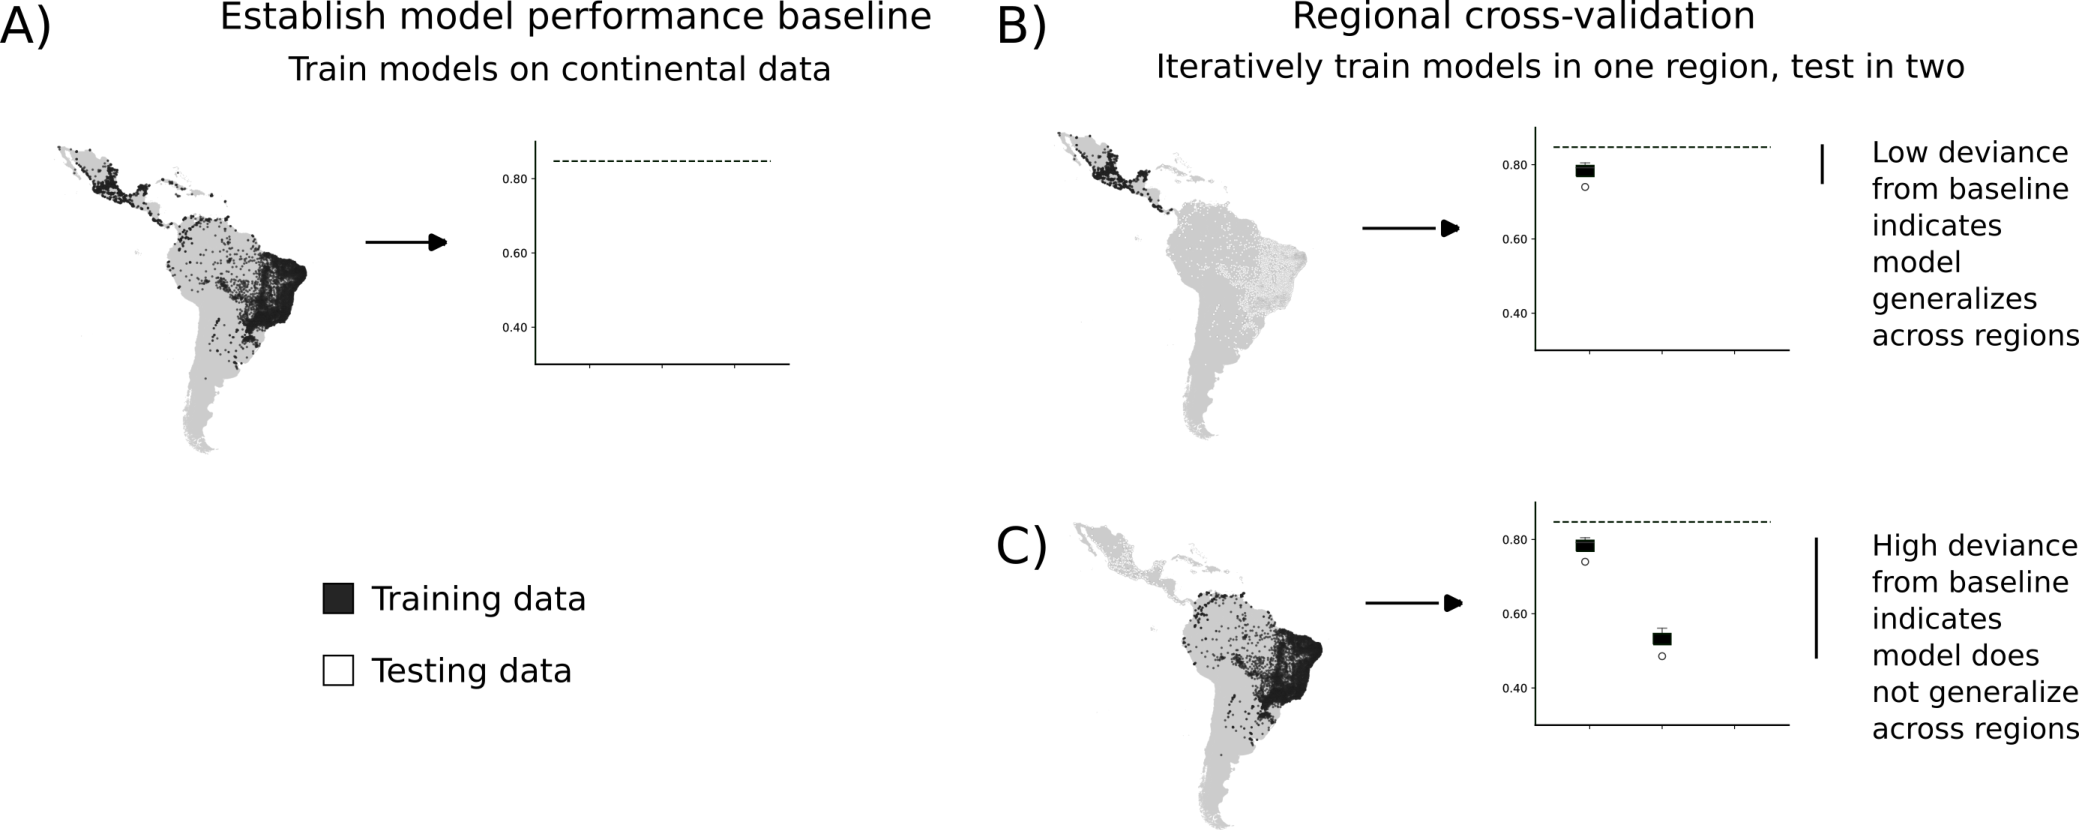
\includegraphics[width=\textwidth]{figures/ch3-cv-conceptual2.pdf}
\centering
\caption[Methods summary for estimating niche conservation.]{Methods summary for estimating niche conservation. A) First we used the species distribution models trained on each set of covariates (per \textit{Section 4.3.2}) to calculate baseline model performance using all occurrence data. B) Then we iteratively trained models using just occurrence records from one of three regions— Mesoamerica, the Caribbean or South America—and tested performance on the remaining two regions. C) Similarity between baseline results and test results indicates that models generalize across regions, providing evidence of niche conservation.}
\label{fig:cv-conceptual}
\end{figure}

\subsection{Spatial Cross-Validation}

To address our third research question, we evaluated evidence for niche conservation in each mosquito vector. In other \textit{Aedes} modeling efforts, this has been done by evaluating model transferability: training SDMs in one region and evaluating how well model predictions transfer to geographically independent regions \cite{Yates2018-hm}. Models that fail to predict occurrence patterns outside the training region have been interpreted to indicate that these vectors are adapting to new climates; that niche shifts are underway, perhaps driven by hidden niche plasticity, which would fundamentally hinder our ability to forecast future distributions \cite{Medley2010-fa, Carlson2016-rc}. However, a few key questions need to be addressed before the results of a model transferability analysis can be interpreted as evidence for or against niche evolution \cite{Liu2020-wk}. These include questions of spatial scale (do the occurrence records span the full extent of covariate space the vector occupies?), sample size (are there enough occurrence records to characterize vector-covariate relationships?) and representation (how well do the environmental covariates selected describe the different dimensions of the vector niche?).

We performed a spatial cross-validation analysis to address these questions. For each vector, the occurrence records were split by geographic region: into records from Mesoamerica, South America and the Caribbean. To quantify the effects of spatial scale, occurrence records from one region were used as training data and the remaining occurrence records were used as test data to evaluate each model. This process was repeated across each region (Fig. \ref{fig:cv-conceptual}). The data were further subsampled within each region via 5-fold cross-validation to evaluate regional model variance and the effects of sample size. To evaluate covariate representation, each model was trained using just covariates from each niche axis (resource availability, temperature, habitat, and precipitation). These models therefore evaluated how well a model trained on a subset of occurrence records from one region transfers to the remaining regions on a per-niche axis basis. 

We used the models trained across the whole study region as our “baseline” model performance for each niche axis. We interpret regional models that approximate baseline performance as evidence of model transferability and therefore as evidence for niche conservatism. The reciprocal is not necessarily true, however. Models that deviate from the baseline are not necessarily evidence of niche evolution; these effects could be driven by issues of spatial scale, sample size or representation.

\begin{figure}[!ht]
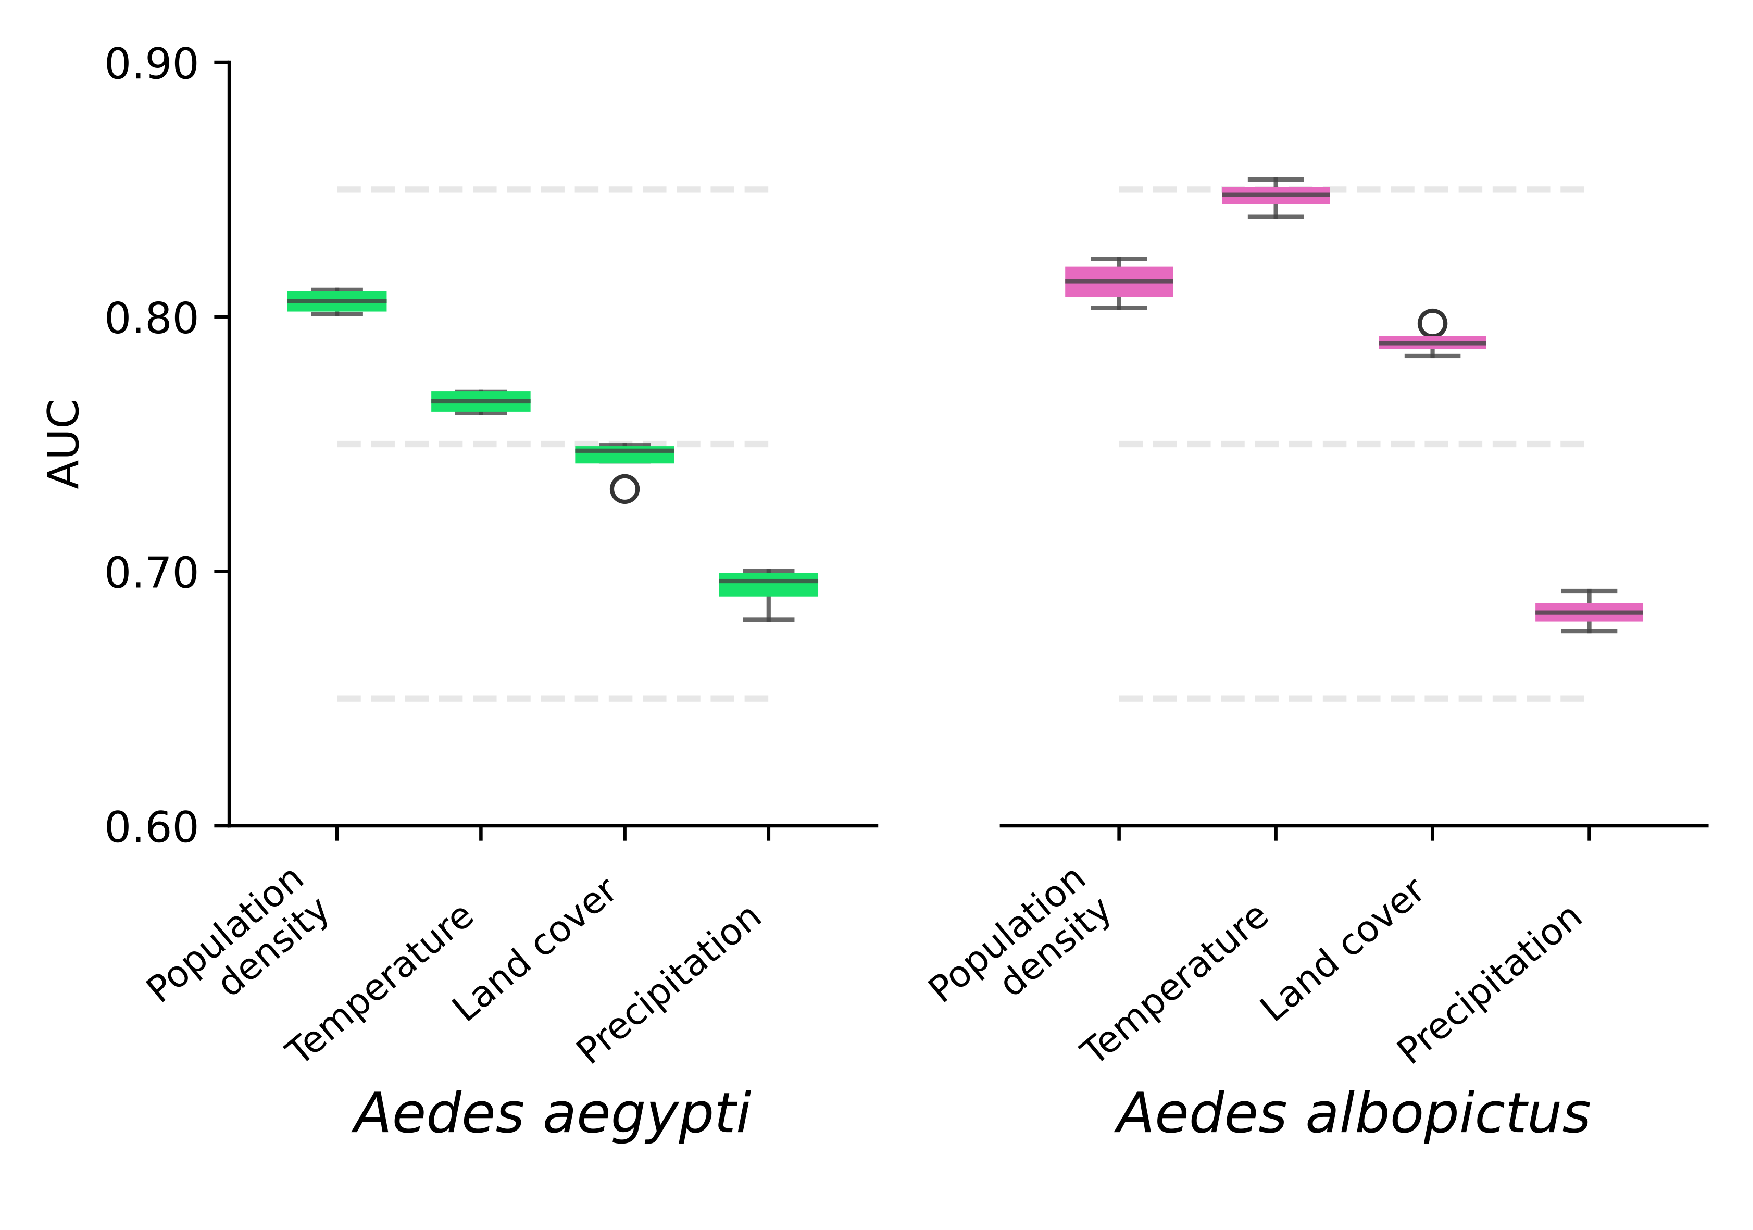
\includegraphics[width=\textwidth]{figures/ch3-importance.pdf}
\centering
\caption[Population density and temperature alone predict \textit{Aedes aegypti} and \textit{Ae. albopictus} occurrence with high precision.]{Population density and temperature alone predict \textit{Aedes aegypti} and \textit{Ae. albopictus} occurrence with high precision. These boxplots compare model performance among species distribution models that were trained on distinct covariate groups. Each set of models was trained only on covariates related to resource constraints (human population density, livestock density), temperature constraints (mean, variance and skewness of daily temperatures), habitat constraints (mean and variance of daily leaf area index, tree cover) or precipitation constraints (mean, variance and skewness of monthly rainfall). Uncertainty estimates were derived from 4-fold jackknifed cross-validation.}
\label{fig:importance}
\end{figure}

\section{Results}

\subsection{Climate, Habitat and Resource Constraints}

\begin{figure}[!ht]
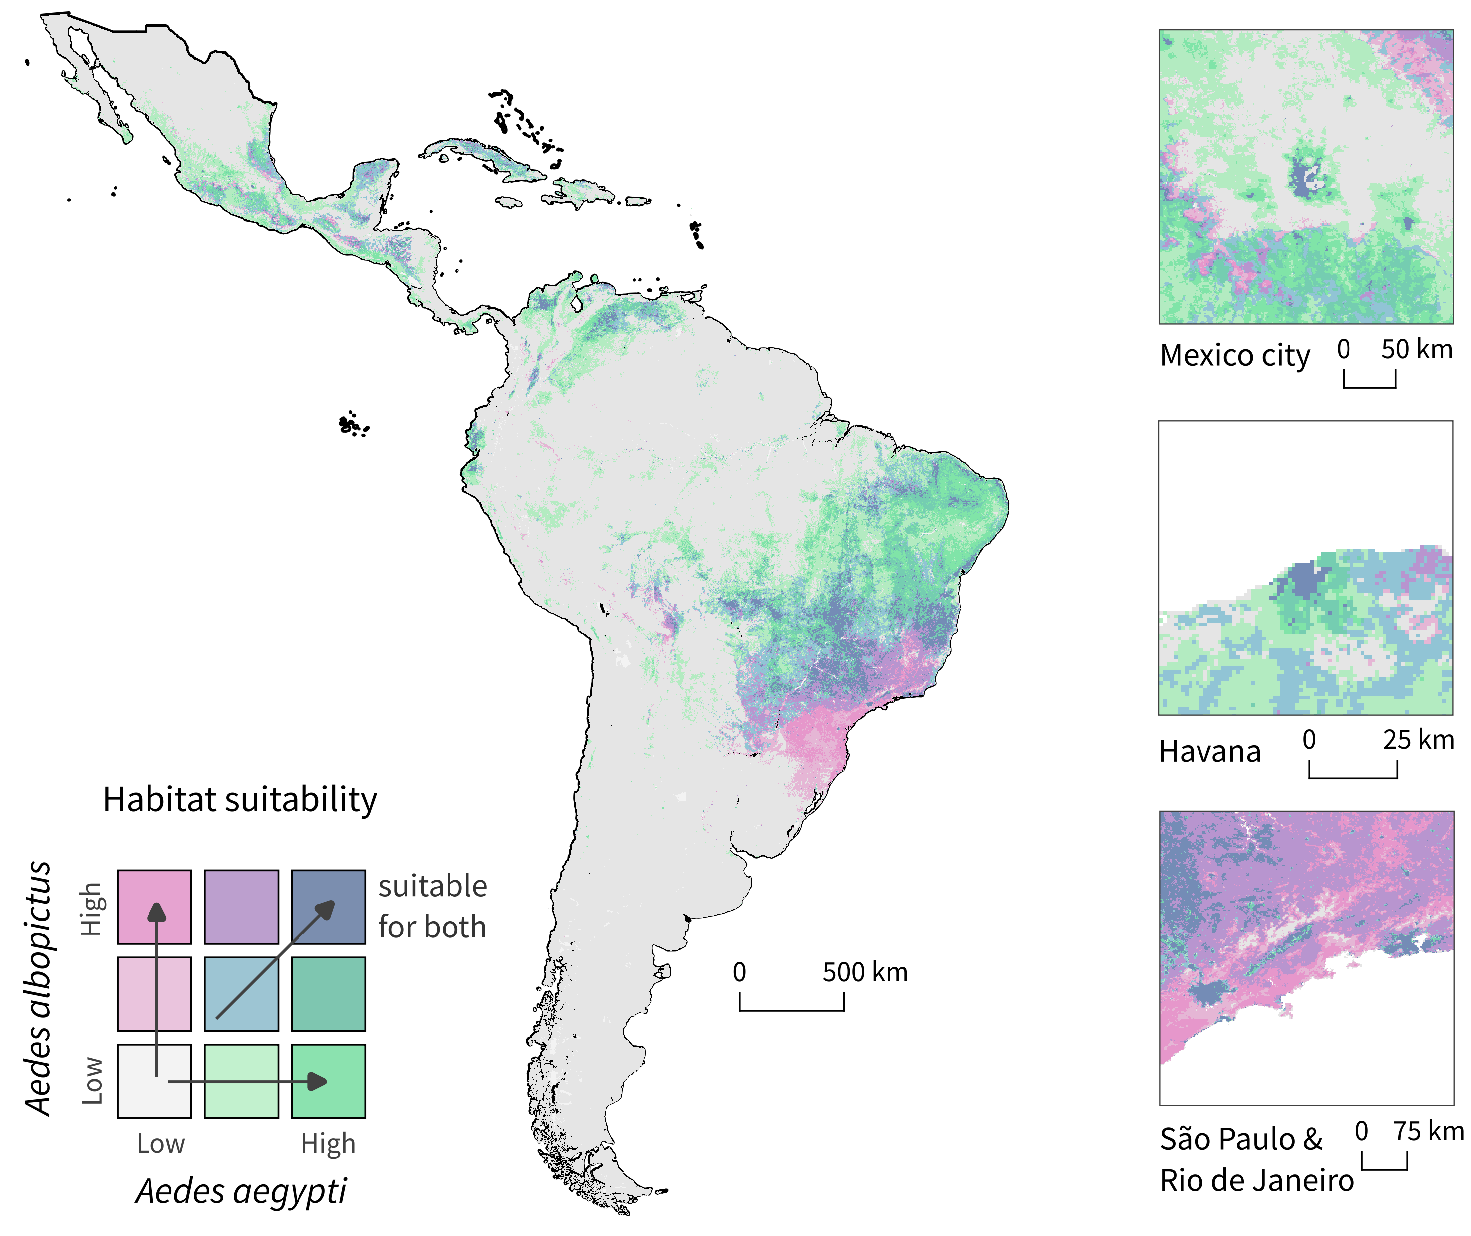
\includegraphics[width=\textwidth]{figures/ch3-map-aedes.pdf}
\centering
\caption[Fundamental niche estimates for each species estimated from the joint model trained on all 11 covariates show overlapping yet distinct fundamental niches for \textit{Ae. aegypti} and \textit{Ae. albopictus} across Latin America and the Caribbean.]{Fundamental niche estimates for each species estimated from the joint model trained on all 11 covariates show overlapping yet distinct fundamental niches for \textit{Ae. aegypti} and \textit{Ae. albopictus} across Latin America and the Caribbean. Insets show niche extents around population centers in Mesoamerica, the Caribbean and South America.}
\label{fig:map-aedes}
\end{figure}

In models that isolated the predictive power of each of the three niche axes alone, we found that resource constraints, characterized by human population density and livestock density, best predicted the realized niche for \textit{Ae. aegypti} (AUC mean = 0.806 $\pm$ 0.004 SD), while temperature constraints best predicted niche patterns for \textit{Ae. albopictus} (AUC mean = 0.847 $\pm$ 0.005 SD; Fig. \ref{fig:importance}). For \textit{Ae. aegypti}, resource constraints were followed by temperature (AUC mean = 0.767 $\pm$ 0.004 SD), land cover (AUC mean = 0.744 $\pm$ 0.007 SD), and precipitation constraints (AUC mean = 0.693 $\pm$ 0.007 SD) in discriminatory power. For \textit{Ae. albopictus}, temperature constraints were followed by resource (AUC mean = 0.814 $\pm$ 0.007 SD), land cover (AUC mean = 0.790 $\pm$ 0.005 SD), and precipitation constraints (AUC mean = 0.684 $\pm$ 0.006 SD) in discriminatory power.

To assess the relative importance of each covariate, and to partially disentangle interactions between drivers, we trained models using all 11 environmental covariates and calculated permutation-based variable importance scores (Table B.2) \cite{Phillips2008-ic}. Human population density was the most important covariate for predicting \textit{Ae. aegypti} distributions (17.9\% of explained permutation variance), and daily temperature variation was the most important covariate for predicting \textit{Ae. albopictus} distributions (51.9\% explained permutation variance). While \textit{Ae. aegypti} models were sensitive to a range of covariates (6 covariates each explained $>$10\% of permutation variance), \textit{Ae. albopictus} models relied on fewer covariates (only 3 covariates each explained $>$10\% of permutation variance). These joint models, trained with all 11 covariates, performed better than any of the single niche-axis models reported above (4-fold cross-validation AUC mean = 0.836 $\pm$ 0.006 SD for \textit{Ae. aegypti}, mean = 0.888 $\pm$ 0.005 SD for \textit{Ae. albopictus}).

The predicted fundamental niche (i.e., potentially suitable habitat) for each vector is widely distributed throughout Central and South America and the Caribbean, particularly in coastal and lowland regions (Fig. \ref{fig:map-aedes}). While many regions are predicted to be suitable for both vectors (Fig. \ref{fig:map-aedes}, blue), distinct regions of high suitability for \textit{Ae. aegypti} (green) or \textit{Ae. albopictus} (pink) were interspersed at small spatial scales (e.g., Havana and Mexico City, Fig. \ref{fig:map-aedes} insets), as well as segregated across larger geographic regions (e.g., São Paulo and Rio de Janeiro for \textit{Ae. albopictus}; the Atlantic dry forest region of Brazil and coastal and lowland regions of Mesoamerica for \textit{Ae. aegypti}; \ref{fig:map-aedes}).

\begin{figure}[!ht]
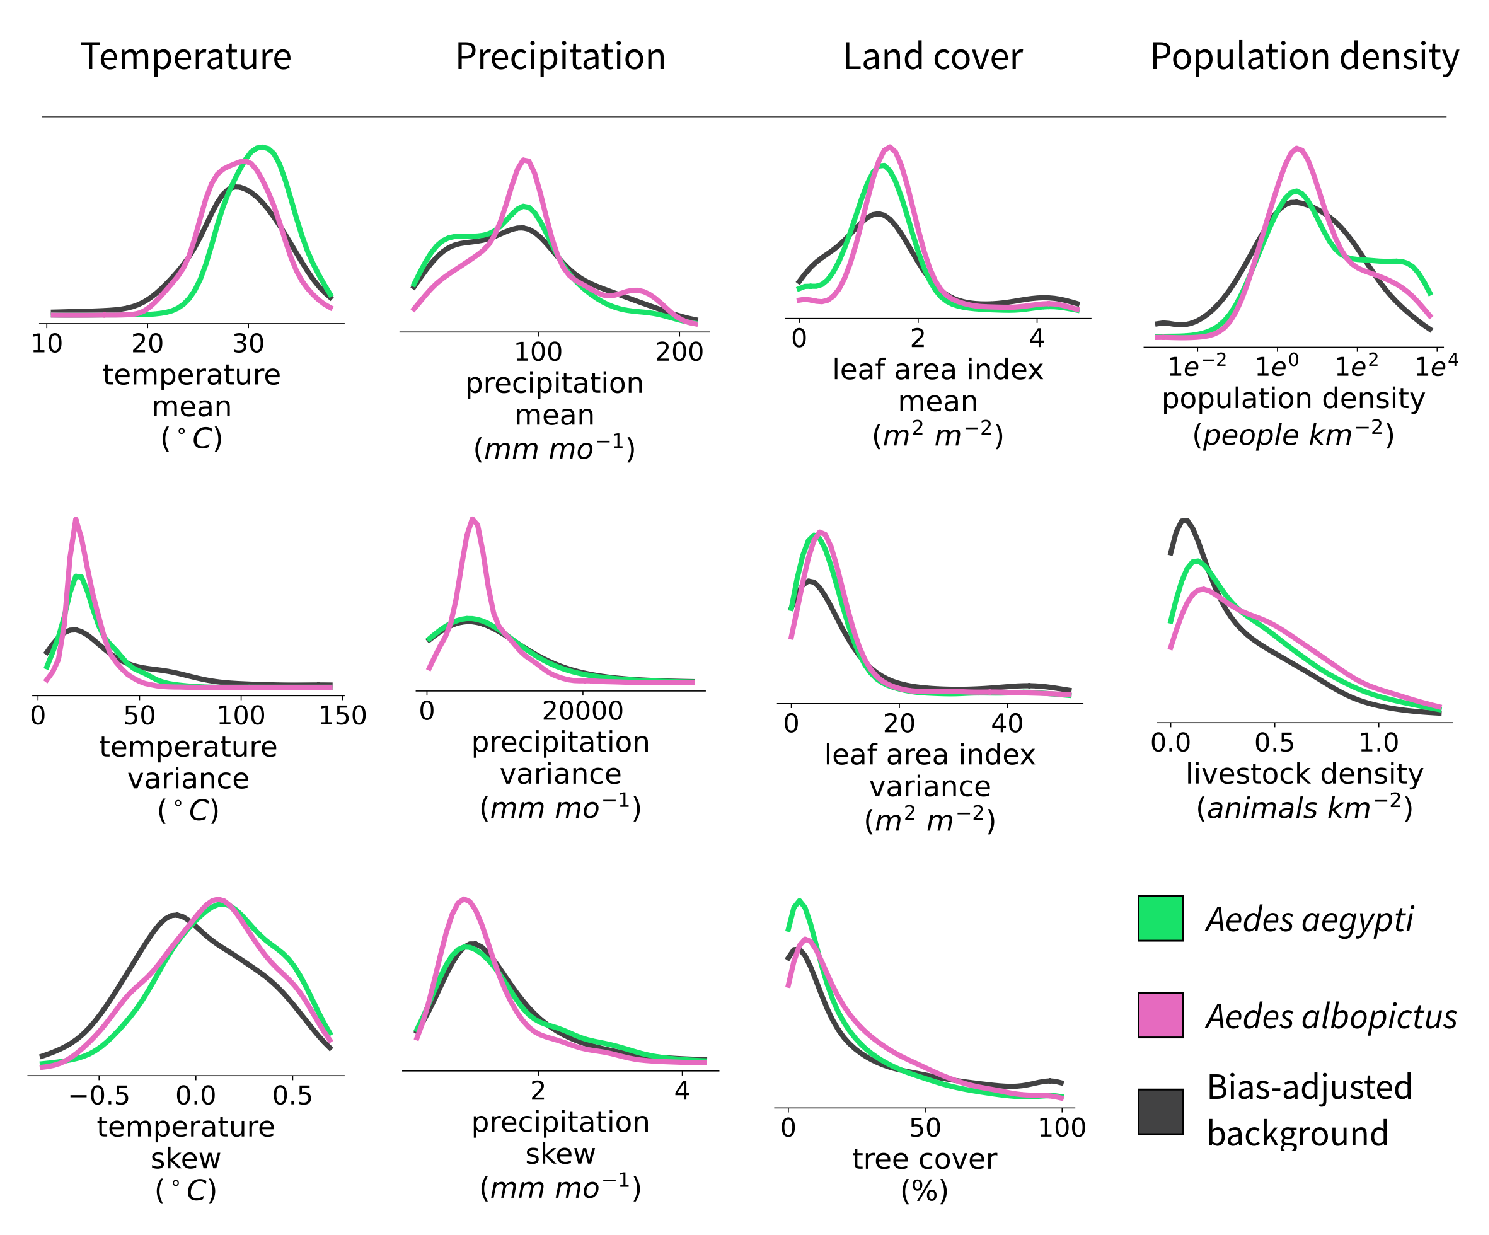
\includegraphics[width=\textwidth]{figures/ch3-density-plots.pdf}
\centering
\caption[Density distribution plots for 11 environmental covariates were extracted from occurrence points for each mosquito species and compared to a bias-adjusted sample of background points across Latin America and the Caribbean.]{\textit{Ae. aegypti} (green) and \textit{Ae. albopictus} (pink) show distinct temperature, precipitation, habitat, and resource use profiles. These density distribution plots for 11 environmental covariates were extracted from occurrence points for each mosquito species and compared to a bias-adjusted sample of background points across Latin America and the Caribbean (grey). Differences between occurrence and background points indicate niche preferences for each species.}
\label{fig:density-plots}
\end{figure}

\subsection{Comparison to Lab and Field Observations}

Both vectors occupied a narrow range of mean daily temperatures (Fig. \ref{fig:density-plots}), with \textit{Ae. aegypti} occurring in warmer areas (95th percentile range 24.9-37.2$\degree C$, mean = 31.0$\degree C$) than \textit{Ae. albopictus} (95th percentile range 22.1-35.9$\degree C$, mean = 29.1 $\degree C$; signed rank test $P < 0.001$), though \textit{Ae. albopictus} mean daily temperature observations were not significantly different from the background (signed rank test $P = 0.430$). These mean observed daily temperature values are slightly higher than the thermal optima for dengue transmission predicted from a mechanistic model based on laboratory data (29.1$\degree C$ for \textit{Ae. aegypti}, 26.4$\degree C$ for \textit{Ae. albopictus}), within the confidence intervals of the thermal optima for fecundity (29.6$\degree C$ for Ae. aegypti, 29.4$\degree C$ for \textit{Ae. albopictus}, and slightly cooler than the predicted optima for biting rates (33.8$\degree C$ for \textit{Ae. aegypti}, 31.8$\degree C$ for \textit{Ae. albopictus} (all based on trait thermal performance data summarized in \cite{Mordecai2017-tb}). Both vectors were observed in areas with significantly lower variance and higher skewness in daily temperatures than the background (all signed rank tests $P < 0.001$), indicating niche preferences for stable thermal conditions skewed towards warm extremes. All significance tests for stochastic equality were performed using the two-sided, nonparametric Brunner-Munzel test \cite{Brunner2000-hd}.

Mosquito abundance data from Perú and Costa Rica were grouped as forest/forest edge (36 sites), agriculture (46 sites) or urban (52 sites) to evaluate niche preferences and abundance patterns along a land use gradient. \textit{Aedes} individuals were more abundant in urban sites than in agriculture or forest/forest edge sites (Table B.3). We identified 156 out of 1,860 mosquitoes collected in urban sites as \textit{Ae. aegypti} or \textit{Ae. albopictus} (8.4\% of individuals), occupying 76.5\% and 62.9\% of urban sites in Costa Rica and Perú, respectively. In agricultural sites, 34 out of 3,128 mosquitoes collected (1.1\% of individuals) were identified as \textit{Ae aegypti} or \textit{Ae. albopictus}. Occupancy rates in agriculture sites varied by country, with 50\% of sites occupied by \textit{Ae. albopictus} in Costa Rica and 8.8\% of sites occupied by \textit{Ae aegypti} in Perú. We identified 9 out of 1,977 mosquitoes collected in forest/forest edge sites as \textit{Ae aegypti} or \textit{Ae. albopictus} (0.5\% of individuals), occupying 27.3\% of forest/forest edge sites in Perú but none in Costa Rica. \textit{Ae aegypti} was the only vector of interest identified in the Perú sites and \textit{Ae. albopictus} was the predominant vector of interest identified in the Costa Rica sites.

\begin{figure}[!ht]
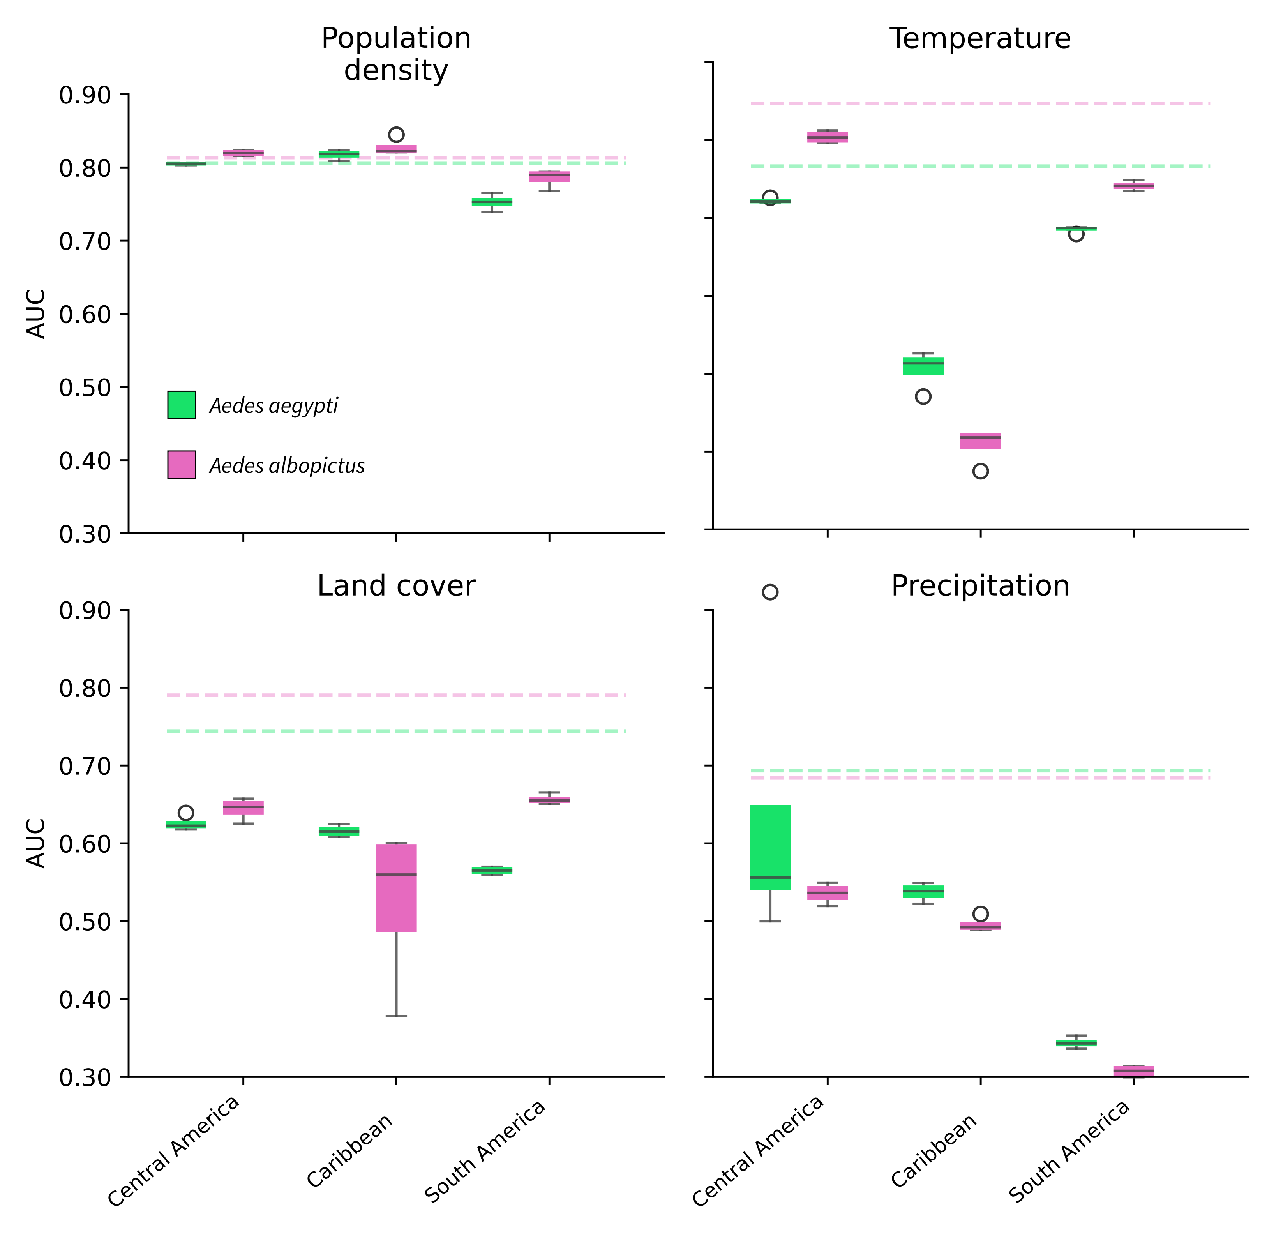
\includegraphics[width=\textwidth]{figures/ch3-cv-results.pdf}
\centering
\caption[Spatial cross-validation analysis showing models trained on just resource use covariates—human population density and livestock density—generalize across regions for both \textit{Ae. aegypti} and \textit{Ae. albopictus}.]{Spatial cross-validation analysis shows that models trained on just resource use covariates—human population density and livestock density—generalize across regions for both \textit{Ae. aegypti} (green) and \textit{Ae. albopictus} (pink; top left panel). By contrast, models trained on temperature (top right), land cover (bottom left), and precipitation (bottom right) on individual regions did not generalize to the remaining areas.}
\label{fig:cv-results}
\end{figure}

These field results corroborate the SDM results, where both vectors were observed in areas with dense human and livestock populations. \textit{Ae. aegypti} was observed in areas with higher human population densities (mean = 632.2 $people\, km^{-2}$) than \textit{Ae. albopictus} (mean = 363.6 $people\, km^{-2}$), both of which were higher than the background (mean = 157.8 $people\, km^{-2}$, signed rank tests $P < 0.001$). \textit{Ae. albopictus} was found in areas with higher livestock densities (mean = 4.4 $animals\, km^{-2}$) than the background (mean = 2.8 $animals\, km^{-2}$, signed rank test $P < 0.001$). Regarding habitat use, mean leaf area index patterns for \textit{Ae. aegypti} were not significantly different from the background (signed rank test $P = 0.961$), but mean leaf area index and tree cover patterns for \textit{Ae. albopictus} were significantly different from the background (signed rank test $P < 0.001$). Both vectors appear to avoid dense forests (95th percentile range 0.0-87.4\% tree cover for \textit{Ae. aegypti} and 0.1-86.1\% tree cover for \textit{Ae. albopictus}).

\subsection{Niche Conservation}

Models trained on just resource constraints within each region (Mesoamerica, the Caribbean, or South America) generalized well across other regions for both vectors (AUC mean range = 0.752-0.827 for both vectors in all regions, based on spatially-jackknifed cross-validation), suggesting consistent resource use patterns across the study area (Fig. \ref{fig:cv-results}). Temperature preferences generalized well for both vectors when trained on occurrence records from just Mesoamerica (AUC mean = 0.722 for \textit{Ae. aegypti}, AUC mean = 0.804 for \textit{Ae. albopictus}) or just South America (AUC mean = 0.685 for \textit{Ae. aegypti}, AUC mean = 0.742 for \textit{Ae. albopictus}), but did not generalize well for either vector when trained on records from just the Caribbean (AUC mean = 0.506 for \textit{Ae. aegypti}, AUC mean = 0.409 for \textit{Ae. albopictus}). Habitat use patterns did not generalize well across regions for either vector, though the degree to which these patterns did generalize was consistent across vectors and across regions (AUC mean range = 0.524-0.657). Precipitation patterns alone performed no better than random chance in most analyses (AUC mean range = 0.307-0.633).

\section{Discussion}

Mechanistically forecasting shifts in vector-borne disease burden with environmental change will be essential to manage and mitigate risks to exposed populations. While climatic constraints on \textit{Aedes} distributions have been well characterized in the lab and by global spatial models, the mechanisms driving habitat and resource constraints were previously poorly characterized. Our results suggest that constraining forecasts based on habitat and resource availability is likely to significantly alter the geography of transmission under global change. We provide evidence that resource constraints (i.e., available blood meals) strongly predict \textit{Aedes} distributions at continental scales, and that vector–resource relationships generalize across regions. Critically, resource constraints intersect with climate and habitat constraints to determine the two species’ ranges, which are overlapping yet distinct. And while \textit{Ae. aegypti} and \textit{Ae. albopictus} are key arbovirus vectors—associated with urbanization, human-made breeding habitats, and human biting—few previous niche modeling studies have explicitly included the density of humans and other blood meal resources as predictive covariates. With human-altered habitats expanding worldwide, the scope of invasion potential for these vectors is dramatic; previous work estimated that 80\% of Brazil’s population already lives in vector-suitable habitat \cite{Cardoso-Leite2014-uq}. And the gap between the fundamental and realized niches for these vectors is shrinking: the southward movement of \textit{Ae. albopictus} has expanded to cover Costa Rica, where it was first officially recorded in northern provinces in the last decade \cite{Calderon_Arguedas2012-bf, Marin_Rodriguez2014-ww}.

Our approach differs from recent \textit{Aedes} niche modeling studies in several regards. First, we exclusively used satellite-derived data as environmental covariates, which are measured continuously along regularly-spaced grids. This is in a fundamentally different data collection strategy from interpolated weather station data, which are sparsely available in Latin America and the Caribbean \cite{Fick2017-am} and widely used by others. By aggregating daily satellite measurements over 16 years, we were able to construct rich, descriptive climate and habitat covariates that track large-scale spatiotemporal variation in each pattern. Second, our method for quantifying and adjusting for sampling bias significantly differs from other \textit{Aedes} niche modeling studies. Since temperature patterns place a physiological limitation on where vectors can survive, researchers often constrain background sample selection to areas within an envelope of thermal viability \cite{Brady2012-tg, Bhatt2013-qa, Kraemer2015-ct}. We instead assumed that, since vector sampling is a key part of epidemiological surveys, sampling bias was driven less by climatic constraints than by disease mitigation priorities in populated areas. We therefore quantified bias using urbanization data, prioritizing background selection from human-dominated areas, as background sampling locations should be selected with the same biases as the occurrence records \cite{Phillips2009-nf, Barbet-Massin2012-pn, Fourcade2018-ws}. Even after controlling for preferential sampling near human populations, we still found that population density and livestock density consistently predicted occurrence patterns, reinforcing the importance of resource constraints in driving vector distributions.

\subsection{Mechanisms of Niche Use}

Our data-driven results are supported by insights from mechanistic relationships between temperature, metabolism and transmission derived from lab tests for both vectors \cite{Mordecai2017-tb, Mordecai2019-ya}. First, daily temperature patterns strongly predict niche use for both species, independently predicting occurrence patterns and driving model sensitivity in multivariate models (Fig. \ref{fig:importance}, Table \ref{tab:sensitivity-analysis}). Second, the density distributions of mean daily temperature are unimodal and peak between 29$\degree C$ for \textit{Ae. albopictus} and 31$\degree C$ for \textit{Ae. aegypti} (Fig. \ref{fig:density-plots}), which is similar to but slightly higher than the mechanistically predicted optima for dengue transmission of 26$\degree C$ and 29$\degree C$, respectively \cite{Mordecai2017-tb}. Third, \textit{Ae. aegypti} is more frequently observed at warmer temperatures than \textit{Ae. albopictus}, tracking warmer thermal optima predicted for biting rates and immature survival rates. However, because these suitable temperatures are widespread in the tropics, including most of Latin America \cite{Brady2012-tg, Ryan2019-pz}, mean temperature alone is not a strong discriminant of \textit{Aedes} occurrence. By contrast, temperature variance strongly predicted occurrence patterns, revealing niche preferences for a narrow envelope of thermal conditions amenable to year-round survival and biting.

Vegetation patterns better predicted the occurrence of \textit{Ae. albopictus}, traditionally considered a more rural vector, than they did \textit{Ae. aegypti}, typically an urban vector (Fig. \ref{fig:importance}). Within areas with suitable breeding habitats and access to blood meal hosts, vegetation provides more suitable microclimates, adult resting habitat, and nectar sources for sugar feeding to support metabolism \cite{Marinotti1990-vx, Martinez-Ibarra1997-ra, Chen2015-dw}. Our vector surveys and other recent work \cite{Troyo2009-yv, Calderon-Arguedas2015-sz} have identified agricultural areas and their adjacent forest elements as key breeding sites for \textit{Ae. albopictus}, including coffee, palm, and pineapple plantations in Costa Rica, and for \textit{Ae. aegypti}, as well as and areas outside mining camps in Perú. The species distribution models capture these niche preferences for areas with low to moderate tree cover and mean leaf area index, combined with high variance in leaf area index, an indicator of vegetation phenology and seasonal agricultural productivity (Fig. \ref{fig:density-plots}).

\subsection{Mechanisms of Niche Conservation}

We found strong evidence for niche conservation in resource use patterns via spatially-explicit cross-validation (Fig. \ref{fig:cv-conceptual}). Models trained on just human population density and livestock density generalized well across regions, suggesting that these vectors have consistent resource requirements that explain spatial distribution patterns better than climate alone. \textit{Ae. aegypti} occurred in higher population densities (mean = 632 $people\, km^{-2}$) than \textit{Ae. albopictus} (mean = 363 $people\, km^{-2}$), both of which were higher than background values (mean = 158 $people\, km^{-2}$). This supports the characterization of \textit{Ae. aegypti} as an “urban-affiliated” species (though it may be more precise to characterize them as “human-affiliated”). While \textit{Ae. albopictus} also preferred human-dominated landscapes, sensitivity analysis showed that their occurrence records were better explained by livestock density (Table B.3). This is consistent with their weak but non-discriminating human biting habits \cite{Gratz2004-xn, Paupy2009-ft, Kamgang2012-sr}. Supplementing human blood meals with livestock blood meals is potentially an effective resource use strategy: livestock is the largest pool of mammal biomass worldwide, and their abundance and geographic footprint is increasing across the region \cite{Bar-On2018-vj, Nepstad_2017-ar, Gilbert2018-bm}, especially as cattle ranching expands in Brazil under the current presidential administration \cite{Rochedo2018-mf, Kroger2020-ys}. This generalist resource use strategy may, in part, explain their invasion dynamics. The spread of \textit{Ae. albopictus} across Latin America and the Caribbean, first reported in Texas and Brazil in the 1980s \cite{Moore1997-of, Santos2003-jy}
—the epicenters of dispersal \cite{Tatem2006-qu, Wagman2013-cx, Ortega-Morales2016-jd}—also coincided with the dramatic expansion of pastures across the region \cite{Geist2002-yo, Barbier2004-sv, Graesser2015-gq}.

We did not see that niche preferences for temperature, land cover, or precipitation generalized across regions, which corroborates the results of similar studies \cite{Medley2010-fa, Pech-May2016-vs, Carlson2016-rc}. However, we do not interpret this as evidence for niche evolution. Instead, we posit that vector–climate and vector–habitat relationships are complex and sensitive to a broad range of environmental variation, which are difficult to fully characterize over small geographic extents using statistically-driven SDMs. This may explain why temperature-driven models trained in the climatically diverse region of South America generalized well to Mesoamerica and the Caribbean, but models trained in the Caribbean were not reciprocal. We suggest that previous evidence for niche evolution may have been driven by this phenomenon and—critically— due to not accounting for niche conservation in resource use patterns, which did generalize. Given these shortfalls, it is important to develop spatial modeling methods based on generalized, mechanistic vector–environment relationships. Our statistically-driven approach provided support for well-known vector–climate relationships, identified new vector–resource mechanisms driving distributions, and highlighted how the generality of vector–habitat relationships remains uncertain.

\section{Conclusion}

As both \textit{Ae. aegypti} and \textit{Ae. albopictus} prefer populated areas in warm climates with low to moderate vegetation cover, directional shifts under global environmental change are likely to expand the range of suitable vector habitat \cite{Ryan2019-pz}. We show here that it is critical to put people on the map in these global change scenarios \cite{Ellis2008-xj}, not only to characterize exposure and vulnerability to vector-borne disease but to better understand shifts in vector populations themselves and to design effective mitigation strategies. We also identified that cattle ranching may present an under-recognized risk driving \textit{Ae. albopictus} invasion and potential arbovirus transmission, which is also forecast to expand in extent in the coming years. With dramatic global environmental changes rapidly approaching, public health planners should be prepared for a potentially devastating expansion of \textit{Aedes} vectors and their arboviral passengers.

\clearpage